% !TeX root = ./main.tex

% TEMPLATE thesis UniPD

\documentclass[a4paper,12pt]{memoir} % memoir is book with abstract support


%%%%%%%%%%%%%%%%%%%%%%%%%%%%%%%%PACKAGES%%%%%%%%%%%%%%%%%%
\usepackage[font=small,labelfont=bf]{caption} %Makes image caption small
\usepackage[a-1b]{pdfx} % Generate a PDF/A

\pdfpagewidth\paperwidth
\pdfpageheight\paperheight

\usepackage[english]{babel} % [english]

\usepackage[utf8]{inputenc}
\usepackage[T1]{fontenc}

\usepackage{lmodern,amsmath,amssymb,graphicx}

% Useful for SI units:
\usepackage[per-mode=fraction,binary-units]{siunitx}

% Useful for bibliography:
\usepackage[style=alphabetic,natbib=false,doi=true,url=false, backend=bibtex]{biblatex}
\addbibresource{Bibliography/bibl}

% If you want to use subsections:
\setsecnumdepth{subsection}

\aliaspagestyle{chapter}{empty} % No page number on new chapter page

% Small margins:
\setulmarginsandblock{3cm}{*}{*}
\setlrmarginsandblock{2cm}{*}{*}
\checkandfixthelayout

\title{Inverse Beta Decay events selection in JUNO using Machine Learning algorithms}
\author{Candidate}
\date{Discussion date}

% METADATA for PDF
\begin{filecontents*}{\jobname.xmpdata}
\Title{Thesis title}
\Author{Candidate}
\Language{en-US} %{en-US}
\Date{YYYY-MM-DD}
\Keywords{keyword1\sep keyqord2\sep keyword3}
\end{filecontents*}

\hypersetup{hidelinks} % Hide link color boxes on pdf


\begin{document}

%%%%%%%%%%%%%%%%%%%%%%%%%%%%%%%%%%%%%% COVER %%%%%%%%%%%%%%%%%%%%%%%%%%%%%%%%%%%%%%
  \frontmatter
  \begin{titlingpage} % titlepage in book
    \vspace{5mm}
    \begin{figure}[ht]
      \centering
      
\includegraphics[scale=.13]{Images/logo.png}
    \end{figure}
    \vspace{5mm}
    \begin{center}
      {{\Large{\textsc{\textbf{UNIVERSITÀ DEGLI STUDI DI PADOVA}}}}\\}
      \vspace{5mm}
      {\textbf{Dipartimento di Fisica e Astronomia}} \\ % Department of XXXXXXXXXXXX
      \vspace{5mm}
      {\textsc{\textbf{Corso di Laurea Triennale in Fisica}}}\\ % Master's Degree in
      \vspace{20mm}
      {\textsc{\textbf{Tesi di Laurea}}}\\ % Final Dissertation
      \vspace{25mm}
      \begin{Spacing}{3}
        {\Large \textbf{\thetitle}}\\
      \end{Spacing}
      \vspace{8mm}
    \end{center}

    \vspace{15mm}
    \begin{Spacing}{1.5}
      \begin{tabular}{p{0.3\textwidth} p{0.3\textwidth} p{0.3\textwidth}}
        Relatore && Laureando\\ % Supervisor && Candidate
        \textbf{prof. Alberto Garfagnini} && \textbf{\theauthor}\\
        Correlatori && \textbf{Badge Number}\\ % Co-supervisors
        \textbf{dott. XXXXXX} && \\ % Dr.
        \textbf{dott. XXXXXX} && \\ % Dr.
      \end{tabular}
    \end{Spacing}
    \vspace{8 mm}
    \begin{center}
      \textbf{Anno Accademico YYYY/YYYY} % Academic Year
          \vspace{5 mm}\\\textbf{\thedate}
    \end{center}
  \end{titlingpage}
  \clearpage{\pagestyle{empty}\cleardoublepage}

%%%%%%%%%%%%%%%%%%%%%%%%%%%%%%%%%%%%%% ABSTRACT %%%%%%%%%%%%%%%%%%%%%%%%%%%%%%%%%%%%%%
  \begin{abstract}
   The Jiangmen Underground Neutrino Observatory (JUNO) will be the largest liquid scintillator-based neutrino detectors in the World, for the next decade. Thanks to its large active mass (20 kt) and state of the art performances (3\% effective energy resolution at 1 MeV), it will be able to perform important measurements in neutrino physics. The proposed thesis will study the application of different Machine Learning inspired algorithms for the discrimination of signal events (interactions of anti-neutrinos coming from the nearby nuclear power plants) from background events.
  \end{abstract}
  \newpage
% If abstract is required also in another language:
% requires: \usepackage[italian, english]{babel}
%   \begin{otherlanguage}{italian}
%     \begin{abstract}
%       Abstract in second language.
%     \end{abstract}
%   \end{otherlanguage}
%   \newpage

%%%%%%%%%%%%%%%%%%%%%%%%%%%%%%%%%%%%%% TABLE OF CONTENTS %%%%%%%%%%%%%%%%%%%%%%%%%%%%%%%%%%%%%%

  \tableofcontents
  \newpage
  %\listoffigures
  %\listoftables

%%%%%%%%%%%%%%%%%%%%%%%%%%%%%%%%%%%%%% BODY %%%%%%%%%%%%%%%%%%%%%%%%%%%%%%%%%%%%%%

  \mainmatter

  \chapter{Introduction}
\section{Neutrinos Oscillation}
The Standard Model of elementary particle interactions provides an accurate description of strong, weak, and electromagnetic interactions, but it treats these interactions as distinct and unrelated. Within this framework, neutrinos are assumed to be massless, but this assumption has been called into question by physicists. Neutrino oscillations, which occur when neutrinos change from one flavor to another, are a potential indication of neutrino mass.\\
The term "neutrino oscillations" refers to this phenomena and it involve the conversion of a neutrino of a particular flavor to another as it propagates through space.

Each known flavor eigenstate, $(\nu_e,\nu_{\mu},\nu_{\tau})$, linked to three respective charged leptons $(e,\mu,\tau)$  via the charged current interactions can be considered a complex combination of neutrino mass eigenstates as follow:

\begin{equation*}
	\left(\begin{array}{l}
		v_e \\
		v_\mu \\
		v_\tau
	\end{array}\right)=U_{\mathrm{PMNS}}\left(\begin{array}{l}
		v_1 \\
		v_2 \\
		v_3
	\end{array}\right)
\end{equation*}
in wich $\nu_i$ are the three mass eigensates, that have 3 masses  $m_i$  $(i = 1,2,3)$, which are non-degenerate, with $m_i \neq m_j$ for $i \neq j$.\\

The matrix $U_{\mathrm{PMNS}}$, called Pontecorvo-Maki-Nakagawa-Sakata (PMNS) matrix, is composed of three rotation matrices, $R_{23}$, $R_{13}$, and $R_{12}$, each corresponding to a different mixing angle, $\theta_{23}$, $\theta_{13}$, and $\theta_{12}$, respectively and a parameter $\delta_{CP}$ called the Dirac CP-violating phase. For this case, the Majorana $C P$ phases are $eta i(i=1,2)$, which are only physically possible if neutrinos are Majorana-type particles and do not participate in neutrino oscillations. Therefore, $U$ can be expressed as:

\begin{equation*} 
	\begin{split}
			U_{\text {PMNS }}&=\\
		=&\left(\begin{array}{ccc}
			1 & 0 & 0 \\
			0 & c_{23} & s_{23} \\
			0 & -s_{23} & c_{23}
		\end{array}\right) \left(\begin{array}{ccc}
			c_{13} & 0 & s_{13} \mathrm{e}^{-\mathrm{i} \delta_{C P}} \\
			0 & 1 & 0 \\
			-s_{13} \mathrm{e}^{\mathrm{i} \delta_{C P}} & 0 & c_{13}
		\end{array}\right) 
		\left(\begin{array}{ccc}
			c_{12} & s_{12} & 0 \\
			-s_{12} & c_{12} & 0 \\
			0 & 0 & 1
		\end{array}\right)\left(\begin{array}{ccc}
			\mathrm{e}^{\mathrm{i} \eta_1} & 0 & 0 \\
			0 & \mathrm{e}^{\mathrm{i} \eta_2} & 0 \\
			0 & 0 & 1
		\end{array}\right)
	\end{split}
\end{equation*}

The theoretical framework for neutrino oscillations involves the calculation of the oscillation probability as a function of the distance traveled by the neutrino, the neutrino mixing matrix, and the difference in squared masses between the three neutrino mass states, $\Delta m_{ij}^2$. Specifically,two nuclear power reactors 53 $\unit{\kilo\meter}$ away from the detector, which mostly produce anti-electron neutrinos $\bar{\nu}_e$ with energy below 10 MeV, are the principal sources of neutrinos for the JUNO experiment. So, it is necessary for the JUNO experiment to calculate the survival probability $P\left(\bar{\nu}_e \rightarrow \bar{\nu}_e\right)$ of electron antineutrinos.

\begin{equation*}
	P\left(\bar{\nu}_e \rightarrow \bar{\nu}_e\right)=1-\sin ^2 2 \theta_{12} c_{13}^4 \sin ^2\left(\frac{\Delta m_{21}^2 L}{4 \mathcal{E}}\right)-\sin ^2 2 \theta_{13}\left[c_{12}^2 \sin ^2\left(\frac{\Delta m_{31}^2 L}{4 \mathcal{E}}\right)+s_{12}^2 \sin ^2\left(\frac{\Delta m_{32}^2 L}{4 \mathcal{E}}\right)\right]
\end{equation*}

where $s_{i j} \equiv \sin \theta_{i j}, c_{i j} \equiv \cos \theta_{i j}, \mathcal{E}$ is the neutrino energy, $L$ the travelled distance and $\Delta m_{i j}^2 \equiv m_i^2-m_j^2$. \\
Past experiments have already given estimates for  $\Delta m_{21}^2,\left|\Delta m_{31}^2\right|$ and the  3 mixing angles.


\begin{figure}[h]
	\centering
	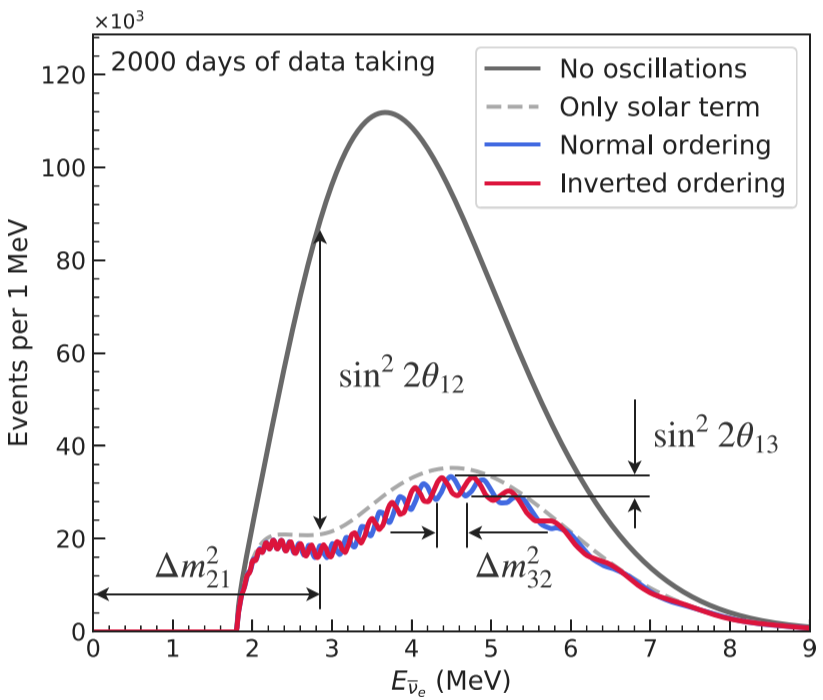
\includegraphics[width=0.4\linewidth]{Images/antineutino_to_antineutrino_probability_plot}
	\caption{JUNO's reactor antineutrino energy spectrum is shown with and without the effect of neutrino oscillation. The gray dashed curve includes only the term in the disappearance probability modulated by $sin^2(2\theta_{12})$, while the blue and red curves use the full oscillation probability for normal and inverted mass orderings. Spectral features driven by oscillation parameters are illustrated, highlighting the rich information available in JUNO's high-resolution measurement of the oscillated spectrum.}
	\label{fig:antineutinotoantineutrinoprobabilityplot}
\end{figure}


%TODO: Questo paragrafo da modificare come è scritto, FrMa
The aim of JUNO is then to improve these results, and especially fix the sign of $\Delta m_{31}^2$ by discriminating between two possibilities:\textit{ Normal Ordering} (\textbf{NO}), where $\left|\Delta m_{31}^2\right|=\left|\Delta m_{32}^2\right|+\left|\Delta m_{21}^2\right|$, and if $m_1<m_2<m_3$ we have the so called \textit{ Inverted Ordering} (\textbf{IO}), where $\left|\Delta m_{31}^2\right|=\left|\Delta m_{32}^2\right|-\left|\Delta m_{21}^2\right|$, and $m_3<m_1<m_2$.
In fact, depending on the sign of $\Delta m_{31}^2$, the plot of \ref{fig:antineutinotoantineutrinoprobabilityplot} is minimally different.


\section{The JUNO detector}

The Jiangmen Underground Neutrino Observatory (JUNO) is an experiment that is currently under construction in Southern China, in Jinji town, 43 km to the southwest of Kaiping city. This multipurpose experiment is expected to detect a large number of antineutrinos from nuclear reactors, with most of them originating from the Taishan and Yangjiang nuclear power plants (NPPs). These two plants are located at a baseline of about 52.5 km from the JUNO detector, which was optimized for the best sensitivity to the neutrino mass ordering, and have a combined nominal thermal power of 26.6 $GW_{th}$. JUNO requires knowledge of the unoscillated reactor antineutrino spectrum shape, which is why a specialized small detector named TAO will be situated approximately 30 meters from one of the Taishan reactors to precisely measure it. The data collected by TAO will serve as a data-driven input to restrict the spectra of the other reactor cores.\\


The JUNO detector comprises three main components, namely the Central Detector (CD), a water Cherenkov detector, and a Top Tracker (TT). The CD is a liquid scintillator (LS) detector, featuring an effective energy resolution of $\sigma_E/E =3\% / \sqrt{E (MeV)}$. It is composed of a 20 kton LS, enclosed within a spherical acrylic vessel, submerged in a water pool, that has a diameter of 43.5 m and a height of 44 m, providing sufficient buffer in all directions to protect the LS from the surrounding rock radioactivity. The water pool contains PMTs, which detect the Cherenkov light emitted from cosmic muons, acting as a veto detector.
The vessel is supported by a stainless steel (SS) structure, via Connecting Bars, with CD Photomultiplier Tubes (PMTs) installed on the inner surface of the SS structure. 
Compensation coils are mounted on the SS structure, aimed at suppressing the Earth's magnetic field and reducing its impact on the photoelectron collection efficiency of the PMTs. 
Atop the water pool lies a Top Tracker, which comprises a plastic scintillator array designed to precisely measure muon tracks. The CD is connected to the outside through a chimney, which facilitates calibration operations. The Calibration House, located above the chimney, contains special radioactivity shielding and a muon detector.\\

A schematic illustrating the location of both JUNO and TAO is shown in Fig. \ref{fig:junoschemeexperiment}.

\begin{figure}[h]
	\centering
	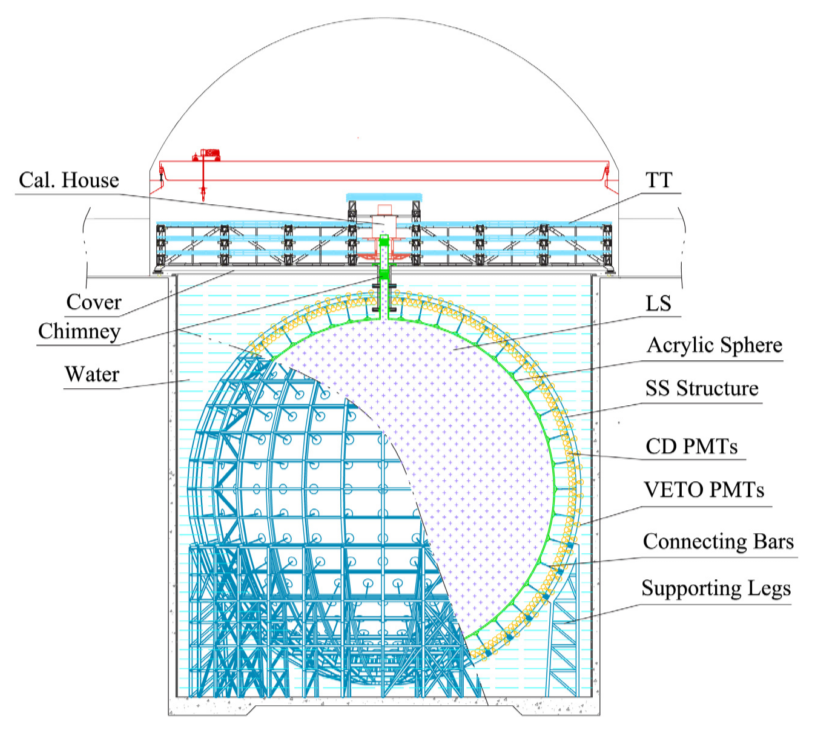
\includegraphics[width=0.7\linewidth]{Images/juno_scheme_experiment}
	\caption[JUNO scheme experiment]{Schematic view of the JUNO experiment}
	\label{fig:junoschemeexperiment}
\end{figure}


\section{JUNO signal and background}
\subsection{Signal}
%LIQUID SCINTILLATOR
The scintillator is doped with a small amount of gadolinium to enhance its sensitivity to antineutrinos via the inverse beta decay (IBD) process. The liquid scintillator used in JUNO is a combination of LAB (linear alkyl benzene) and PPO (2,5-diphenyloxazole) doped with a small amount of bis-MSB (1,4-bis(2-methylstyryl) benzene). When a neutrino interacts with the scintillator, it can produce charged particles such as electrons, protons, and alpha particles that travel through the scintillator and excite the scintillation molecules. This excitation results in the emission of photons with a wavelength of around 430 nm. These photons are detected by 20,000 20-inch photomultiplier tubes (PMTs) distributed in a 3-dimensional arrangement inside the detector.\\




\begin{equation}
	\begin{aligned}
		\overline{\nu}e + p &\rightarrow e^+ + n \\
		n + ^A_ZX &\rightarrow ^{A}_{Z-1}X^* + \gamma \\
		e^+ + e^- &\rightarrow 2\gamma
	\end{aligned}
\end{equation}

The PMTs detect the light and convert it into an electrical signal. The signals from all the PMTs are then combined to reconstruct the position and energy of the original neutrino interaction. This technique allows JUNO to measure the energy of the incoming neutrino to high precision, which is crucial for studying neutrino oscillation.

Moreover, the scintillator's composition and the detector's design are optimized to reduce background noise from other sources of radiation, such as cosmic rays and natural radioactivity. By carefully controlling these backgrounds, JUNO aims to achieve a signal-to-background ratio of better than 1:10,000, which is essential for observing the subtle effects of neutrino oscillation.

In JUNO's location, the energy spectrum will be distorted by two types of oscillations. The first is a slow (low frequency) oscillation driven by $\Delta m_{21}^2$ and modulated by $\sin ^2 \theta_{12}$, while the second is a fast (high frequency) oscillation driven by $\Delta m_{31}^2$ and modulated by $\sin ^2 \theta_{13}$. Fitting the data spectrum against the predicted spectrum distorted by standard neutrino oscillations enables measuring the oscillation parameters.\\
\subsection{Background}
Several different types of backgrounds signal are produced in the detector. For analysis we deeply analysed only the three most important contributes:


\paragraph{Radiogenic Backgrounds}

Radiogenic backgrounds arise from decays of radioactive isotopes in detector materials and surrounding rock. These decays can produce various forms of radiation, such as gamma rays and neutrons, which can interact with the detector and produce background events. Examples of radiogenic isotopes include $^{238}\mathrm{U}$, $^{232}\mathrm{Th}$, $^{40}\mathrm{K}$, and their daughter products. The main contributions to the radiogenic backgrounds come from the $^{238}\mathrm{U}$ and $^{232}\mathrm{Th}$ decay chains, with a smaller contribution from $^{40}\mathrm{K}$.

\paragraph{Cosmogenic Backgrounds}

Cosmogenic backgrounds arise from interactions of cosmic rays with materials surrounding the detector, such as the atmosphere and the Earth's crust. Muons produced in these interactions can penetrate the detector and produce background events. Specifically they interact with detector materials, producing isotopes such as $^{11}\mathrm{C}$, $^{9}\mathrm{Li}$, and $^{8}\mathrm{He}$, instable atoms which decay and produce additional background events.

\paragraph{Atmospheric Neutrino Backgrounds}

Atmospheric neutrino backgrounds arise from interactions of cosmic ray protons and nuclei with the Earth's atmosphere, which produce a flux of neutrinos that can interact with the detector. These interactions can produce both charged and neutral current events, which can mimic the signal from reactor neutrinos.

\paragraph{Reactor Antineutrino Backgrounds}

Reactor antineutrino backgrounds arise from the neutrinos produced in the nuclear reactors that power the JUNO experiment. These antineutrinos are the main signal for JUNO, but a small fraction of them can interact with the detector in ways that mimic background events. These interactions can produce both charged and neutral current events, which can be difficult to distinguish from the signal.


Here a viasualization sumary of all the bacgrounds contributions:

\begin{figure}[h]
	\centering
	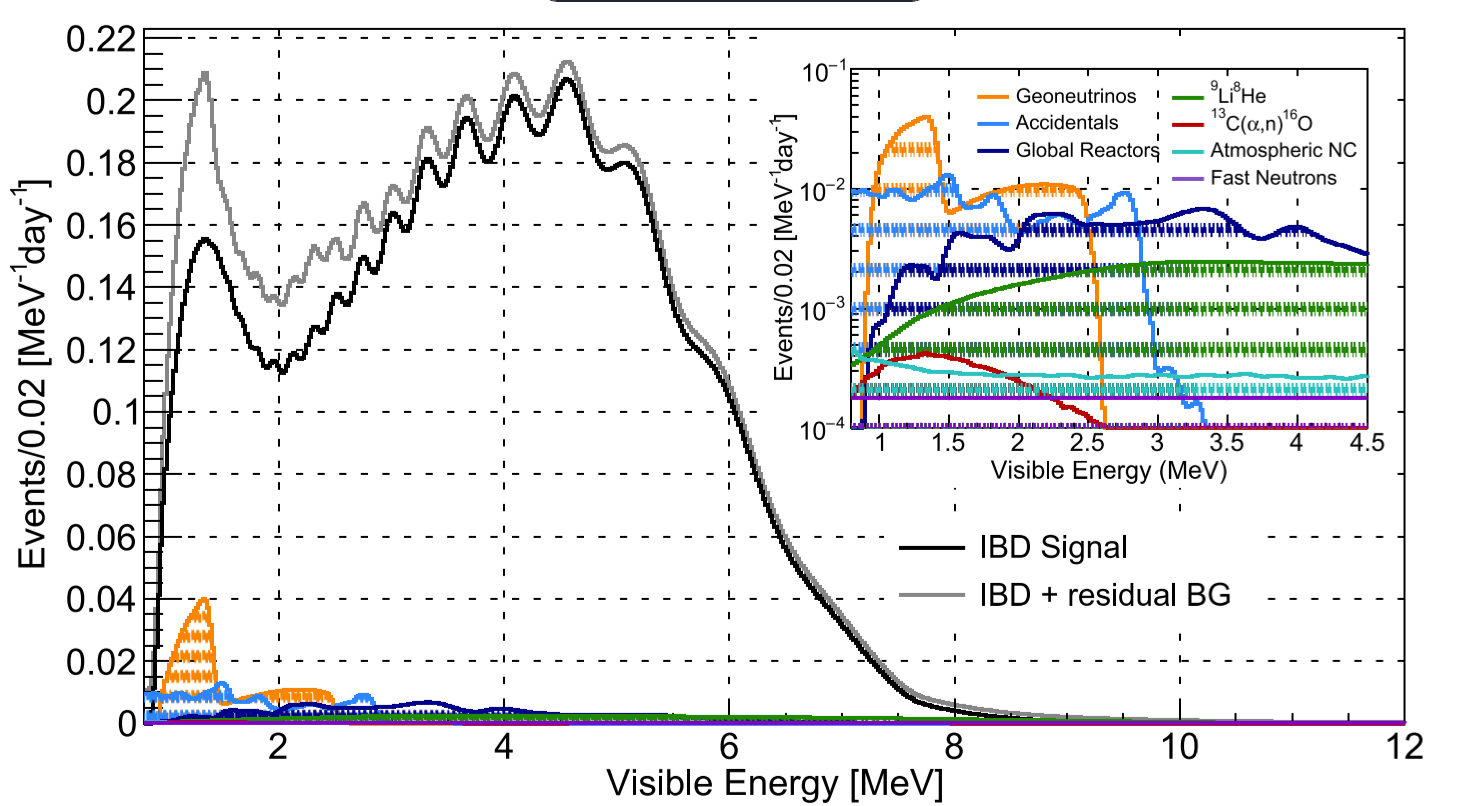
\includegraphics[width=0.7\linewidth]{Images/backgrounds_spectrum}
	\caption{Visible energy spectrum as measured by the LPMT system with (grey) and without (black) backgrounds is that which is anticipated for JUNO. The energy resolution is one of the assumptions listed in the text. The predicted backgrounds, which make up around 7$\%$ of the whole sample of IBD candidates and are primarily confined below, are shown in the inset as spectra. ~ 3 MeV}
	\label{fig:backgroundsspectrum}
\end{figure}

  \chapter{Frameworks}
\section{Introduction to Machine Learning}

Machine learning is a powerful tool that can be used to identify patterns in complex datasets. In the context of particle physics, machine learning algorithms can be used to detect signals from background noise in large datasets generated by detectors. In particular, for the detection of IBD signals from background, machine learning algorithms can be used to identify patterns in the data that are indicative of an IBD event, and to distinguish these signals from the background noise explained above.

\subsection{Supervised Learning}
Supervised learning, a cornerstone of machine learning, operates on the premise of training an algorithm using a labelled dataset. This training ensures that each input aligns with a correct output, with the overarching aim to develop a function that can link input data to output data accurately. A primary task stemming from supervised learning is binary classification, which is responsible for classifying elements of a dataset into one of two possible categories based on inherent features. In the context of this thesis, the emphasis is on applying the binary classification task to the JUNO experiment. The task is to distinguish whether a specific event is an Inverse Beta Decay (IBD) event or a background event.\\
 
Two distinct machine learning algorithms, \textbf{Gradient Boosting Decision Trees} and \textbf{Neural Networks}, are deployed to achieve this.

\section{Decision Tree}
A Decision Tree is a supervised machine learning algorithm used for classification and regression. It segments a dataset into subsets by applying decision rules inferred from the data's features. Each internal node represents a rule, dividing the data into two groups. The choice of rule is based on Information Gain, which relies on Entropy.

Entropy $H$ quantifies the impurity within a set $S$ and is defined as:

\begin{equation}
	H(S) = - p_{+} \log_{2}(p_{+}) - p_{-} \log_{2}(p_{-})
\end{equation}

Here, $p_+$ and $p_-$ denote the proportions of positive and negative instances in the set S, respectively. Entropy attains a maximum value when the set S contains an equal number of positive and negative instances, reflecting the highest uncertainty.

Information Gain (IG) measures the reduction in entropy achieved by partitioning the instances based on a feature (A). It is the difference between the entropy of the set before the split (H(S)) and the weighted sum of the entropies of each subset resulting from the split. It can be formulated as:

\begin{equation}
	IG(S, A) = H(S) - \sum_{v \in V(A)} \left(\frac{|S_v|}{|S|}\right) H(S_v)
\end{equation}

where $V(A)$ indicates the set of all possible values of feature A.\\
In this equation, $S_v$ denotes the subset of instances in S for which the feature A takes on the value v. $|S_v|$ and $|S|$ are the cardinalities of the sets $S_v$ and $S$, respectively.\\

The algorithm constructs the tree by recursively applying these splits, each time selecting the feature that results in the maximum information gain. This process continues until a stopping criterion is met, such as reaching a pre-specified maximum depth of the tree or a minimum number of samples per leaf.\\


While Decision Trees are straightforward and practical models, their ability to decipher complex patterns in data can be limited. This limitation paves the way for a more advanced technique known as Gradient Boosting Decision Trees. 

\subsection{Gradient Boosting Decision Trees}

 %[] https://www.youtube.com/watch?v=PxgVFp5a0E4&ab_channel=Prof.RyanAhmed
Gradient Boosting is a machine learning algorithm that stems from the concept of boosting, with the application of gradient descent methodology. Its goal is to produce a robust predictive model through the combination of multiple weak learners, typically decision trees.

The primary innovation in Gradient Boosting over classical boosting techniques is its approach to error correction. Instead of modifying the weights of misclassified instances, Gradient Boosting fits each new tree to the residuals (or the negative gradient) of the loss function with respect to the prediction of the existing ensemble of trees. This means each new tree is trained to predict the error of the existing model, thereby iteratively reducing the overall error.

Let's formalize this process:

\begin{enumerate}
	\item \textbf{Initialization}: We begin by initializing our model with a constant value. This is denoted as $F_0(x) = \arg\min_{\gamma} \sum_{i=1}^{N} L(y_i, \gamma)$, where $L(y, F(x))$ represents the loss function, $y$ represents the true target value, and $F(x)$ is the model's prediction for the input features $x$. This constant prediction, $\gamma$, is chosen to minimize the total loss over all $N$ instances. Thus, our initial model starts with a prediction that globally minimizes the loss.
	\item \textbf{Computation of Residuals}: Next, we iteratively construct an ensemble of $M$ trees. For each iteration $m=1$ to $M$, we calculate the residuals as
	\begin{equation}
		r_{im} = - \left[\frac{\partial L(y_i, F(x_i))}{\partial F(x_i)}\right]_{F(x)=F_{m-1}(x)}
	\end{equation} 
 	for each instance $i=1,2,...,N$. These residuals are essentially the negative gradients (or first derivatives) of the loss function with respect to the model's predictions. They provide a measure of the direction that would decrease the loss function fastest.
	\item \textbf{Fitting a Decision Tree}: After computing the residuals, we fit a new decision tree, $h_m(x)$, to these residuals. This tree is thus trained to predict the negative gradient of the loss function, using train it using the training set 
	${(x_i, r_{im})}_{i=1}^n$. By doing so, it attempts to correct the errors made by the current ensemble model.
	\item \textbf{Model Update}: The model is then updated by applying the rule
	\begin{equation}
		F_m(x) = F_{m-1}(x) + \nu \cdot h_m(x)
	\end{equation}
 	Here, $\nu$ represents the learning rate, a parameter typically less than 1, which controls the contribution of each tree to the final prediction. This essentially adjusts the previous model's prediction in the direction that most decreases the loss.
	\item \textbf{Final Model}: The final model's prediction is given by $F_M(x) = F_0(x) + \sum_{m=1}^{M} \nu \cdot h_m(x)$. In the final ensemble model, each decision tree provides a small correction to the predictions of the previous trees, collaboratively reducing the loss function's value and improving the overall model's performance.
\end{enumerate}


An advanced and highly efficient implementation of this method is XGBoost, which introduces several improvements such as parallel processing.


\section{Neural Networks}
Neural Networks (NNs) are computational models that draw inspiration from the interconnected structure of the human brain. Each individual computational unit, often referred to as an "artificial neuron" or simply "neuron", is designed to mimic the fundamental working mechanism of a biological neuron.

Let's denote the inputs to an artificial neuron as $ x = [x_1, x_2, ..., x_n] $, a representation analogous to dendrites in a biological neuron. These inputs are linearly transformed by a set of weights, $ w = [w_1, w_2, ..., w_n] $, summed together, and a bias term, $ b $, is added to the result. This operation can be expressed mathematically as:

\[
z = \sum_{i=1}^{n} w_i x_i + b 
\]

The calculated value, $ z $, is then passed through an \textit{activation function}, $ f $, to generate the neuron's output, $ a = f(z) $.


The activation function introduces non-linearity into the model, which is crucial for the network's ability to learn complex patterns. Common choices for $ f $ include the sigmoid, hyperbolic tangent, and ReLU (Rectified Linear Unit) functions.\\

An Artificial Neural Network builds upon the concept of the artificial neuron to form an interconnected assembly of these neurons, structured in layers. An ANN typically comprises an input layer, one or more hidden layers, and an output layer. Each layer may contain one or more neurons, and the layers are fully connected, meaning every neuron in one layer connects with all neurons in the following layer.

The following is a graphical representation of an ANN and a single neuron:

%TODO: Migliorare la qualità dell imagine, eliminare la parte scritta

\begin{figure}[h!]
	\centering
	
	\subfloat[Graphic representation of ANN]{
		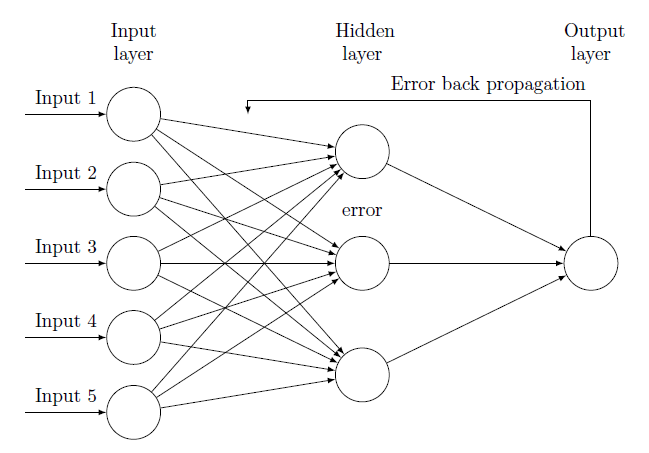
\includegraphics[width = 0.4\textwidth]{Images/fig_neural_network}
		\label{fig:nn_neuron}
	}
	\centering
	\subfloat[Single Neuron representation]{
		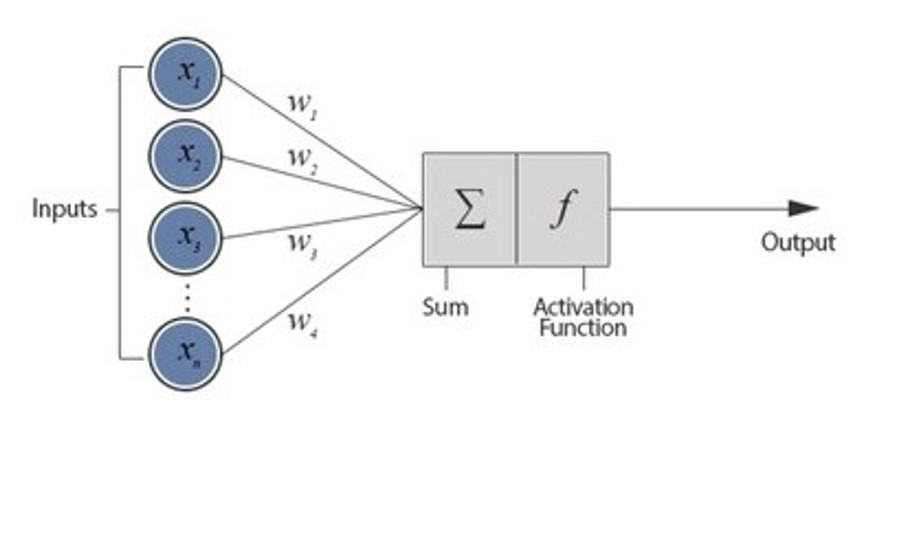
\includegraphics[width = 0.4\textwidth]{Images/nn_neuron}
		

	}
	
\end{figure}


For classification problems, the output layer typically uses a softmax function for multi-class problems to output a probability distribution over the classes, or a sigmoid function for binary classification problems to provide the probability of the positive class.

Training a neural network involves a two-step process: \textit{forward propagation} and \textit{backpropagation}. \\

In \textbf{forward propagation}, the input is passed through the network to generate an output. This output is then compared with the actual target to compute the loss function $ L $.

\textbf{Backpropagation} uses the chain rule of calculus to compute the gradient of $ L $ with respect to the network's parameters, which are then used to update the weights and biases:

\[
\frac{\partial L}{\partial w} = \frac{\partial L}{\partial a} \frac{\partial a}{\partial z} \frac{\partial z}{\partial w}
\]

Here, $ \frac{\partial L}{\partial a} $ is the derivative of the loss function with respect to the activation output, $ \frac{\partial a}{\partial z} $ is the derivative of the activation function, and $ \frac{\partial z}{\partial w} $ is the derivative of the weighted sum with respect to the weights.

Once these gradients are calculated, they are used to update the weights and biases via \textit{gradient descent}, a process that iteratively adjusts the parameters to minimize the loss function:

\[
w_{\text{new}} = w_{\text{old}} - \alpha \frac{\partial L}{\partial w}
\]

\[
b_{\text{new}} = b_{\text{old}} - \alpha \frac{\partial L}{\partial b}
\]

In these equations, $ \alpha $ is the learning rate, a hyperparameter that determines the size of the steps the algorithm takes down the gradient towards the minimum.

The interconnected structure of ANNs, combined with the ability of backpropagation and gradient descent to effectively adjust the model parameters, allows these networks to learn and represent complex, non-linear relationships in the data.

  
%	\input{section/intro}
% 	\input{section/more}
%   \input{section/trials}
%   \input{section/results}
%   \input{section/conclusions}

%%%%%%%%%%%%%%%%%%%%%%%%%%%%%%%%%%%%%% BIBLIOGRAPHY %%%%%%%%%%%%%%%%%%%%%%%%%%%%%%%%%%%%%%

  \backmatter

  \renewcommand{\bibname}{References}
  \nocite{*}
  \printbibliography





\end{document}
